\section{Resultados y análisis}

Se realizó una serie de entrenamientos con las palabras que se deseaban, en este caso son 1) ``lumos'', la cual pretende controlar las luces; 2) ``musica'', el cual pretende controlar un reproductor de música y por último 3) ``tele'', el cual es para controlar un televisor.

\begin{figure}[H]
    \centering
    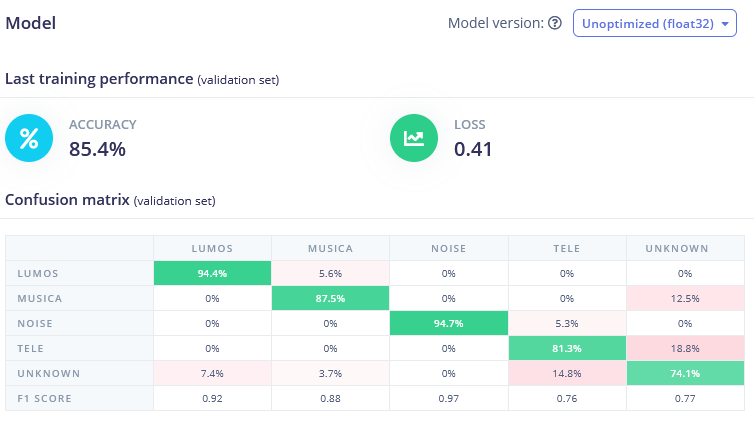
\includegraphics[width=\textwidth]{Imagenes/training.png}
    \caption{Métricas de rendimiento de la red neuronal con datos de validación.}
    \label{valid-data}
\end{figure}

\begin{figure}[H]
    \centering
    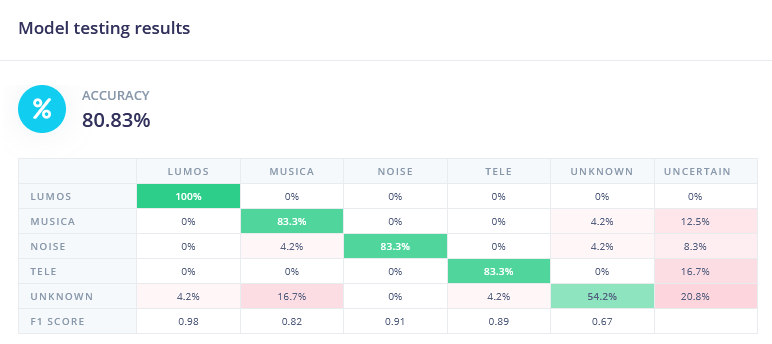
\includegraphics[width=\textwidth]{Imagenes/testing.png}
    \caption{Métricas de rendimiento de la red neuronal con datos de prueba.}
    \label{test-data}
\end{figure}

Como se muestra en las figuras \ref{valid-data} y \ref{test-data}, 
se observa que la precisión del modelo es del 85.4\% y 80.83\% con los datos de validación y de prueba, respectivamente. Esta precisión es más bajo que la precisión que el \href{https://docs.edgeimpulse.com/docs/tutorials/end-to-end-tutorials/responding-to-your-voice}{tutorial} de Edge Impulse obtuvo. Una principal razón se debe a que en el tutorial grabó 10 minutos de cada comando así como 10 minutos de ruido. En cambio, en este laboratorio se grabó 2 minutos de cada comando y ruido.


En la siguientes figuras se observa los resultados en el Thingsboard, es decir, haciendo uso de las palabras claves para realizar una tarea.
En la primera prueba, se utilizó la palabra ``lumos'', con el fin de poder controlar las luces,  como se puede observar en la figura \ref{lumos}.

\begin{figure}[H]
    \centering
    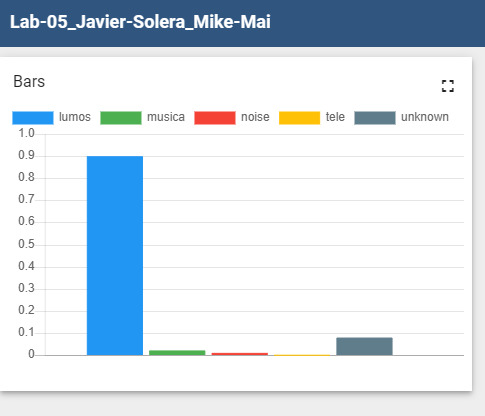
\includegraphics[width=\textwidth]{Imagenes/lumos.jpg}
    \caption{Prueba con la palabra ``lumos''.}
    \label{lumos}
\end{figure}

Como se puede observar, se obtuvo un respuesta del programa muy satisfactoria, ya que una vez que se dice la palabra lumos, el Arduino detecta que se esta diciendo esta palabra, mientras que las demás palabras y ruidos se mantienen bajos.

Luego se realizo una prueba con la palabra musica, con el fin de simular de encender un reproductor de musica, en la figura \ref{Musica} se observa lo que sucede cuando uno le dice al Arduino la palabra clave ``musica''.

\begin{figure}[H]
    \centering
    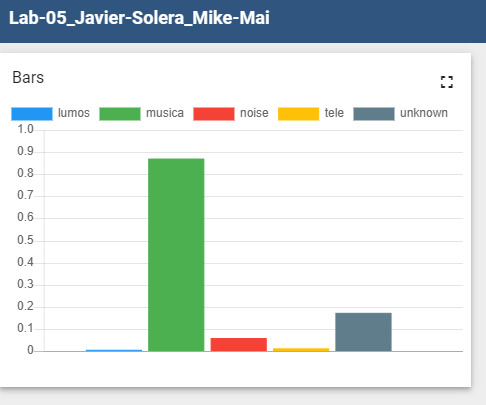
\includegraphics[width=\textwidth]{Imagenes/musica.jpg}
    \caption{Prueba con la palabra ``musica''.}
    \label{Musica}
\end{figure}

Se puede observar que la señal con la etiqueta ``Musica'' se levanta y las demás se mantienen abajo, también se observa que la etiqueta de ruido se levanta un poco y esto se debe a que probablemente detecto un mínimo de ruido en el momento de la ejecución, lo mismo con el ``unknown''.

Luego, se realizó una prueba con la palabra calve ``tele'', el cual pretende simular el encendido de un televisor en una casa.

\begin{figure}[H]
    \centering
    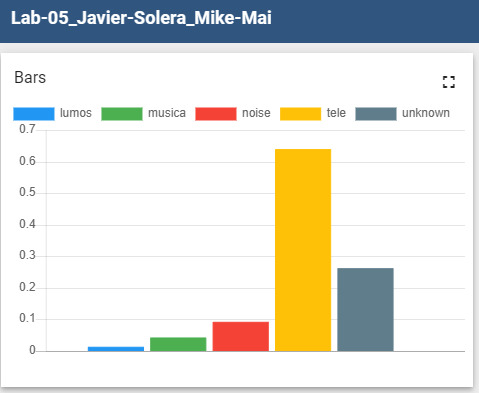
\includegraphics[width=\textwidth]{Imagenes/tele.jpg}
    \caption{Prueba con la palabra ``tele''.}
    \label{tele}
\end{figure}

Como se observa en la figura \ref{tele}, la barra amarilla se levanta, dando a entender que el sistema comprendió muy bien la palabra ``tele'', la cual era la que se deseaba utilizar, también se levanta el ``unknown'' y esto es porque probablemente detectó ciertas voces distintas a las nuestras. 

Luego se midió el ruido, el cual se ve reflejado en la figura \ref{noise}, el cual en esta medición se toma todo lo que se considera ruido ambiental, es decir, ruido de la calle, de electrodomésticos utilizándose, etc. 

\begin{figure}[H]
    \centering
    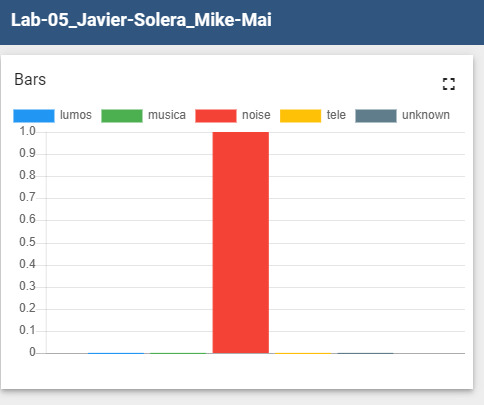
\includegraphics[width=\textwidth]{Imagenes/noise.jpg}
    \caption{Prueba con ruido de ambiente.}
    \label{noise}
\end{figure}

Luego se realizo una medición de distintas voces, de manera para comprobar el funcionamiento y reconocimiento de voz del programa.

\begin{figure}[H]
    \centering
    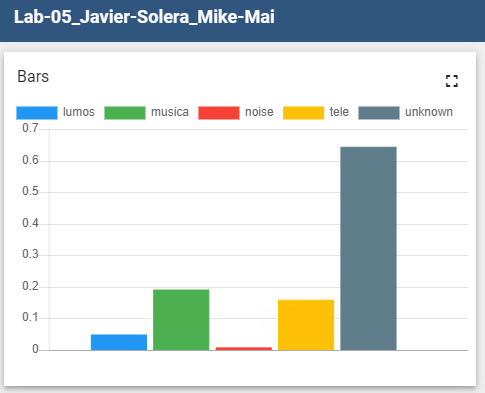
\includegraphics[width=\textwidth]{Imagenes/unknown.jpg}
    \caption{Prueba con voces o palabras diferentes.}
    \label{unknown}
\end{figure}

Tanto los datos de ruido y los datos de ``unknown'' son necesarios para tener un entrenamiento bueno y satisfactorio y así tener un mejor funcionamiento a la hora de detectar las palabras claves, ya que así se puede entrenar la red neuronal y así se puedan ejecutar las acciones que se desean cuando se dicen las palabras claves (`` lumos'', ``tele'' y ``musica''). Cabe destacar que el Arduino con el modelo nunca tuvo ni tendrá una precisión del 100\% al detectar palabras. Es más, durante las pruebas se tuvo que repetir varias veces cada comando para que eventualmente el modelo capture el comando y clasifique correctamente el comando. Las figuras \ref{lumos}, \ref{Musica}, \ref{tele}, \ref{noise} y \ref{unknown} solo muestra el caso cuando se clasifica correctamente. 





































